\documentclass[11pt]{article}
\usepackage[margin=0.82in]{geometry}
\usepackage{amsmath,amssymb,booktabs,graphicx,array,xcolor,xurl,hyperref}
\usepackage[T1]{fontenc}
\newcommand{\NA}{\textemdash}
\title{Stationary-autocorrelation audit of the three-mode relaxation rate}
\author{}
\date{7 September 2026}
\begin{document}
\maketitle

\section*{Question and verdict}
We replaced the window-dependent fit of conditional expectations by stationary
autocorrelations
\[
 C_g(t)=\langle g(X_s)g(X_{s+t})\rangle_s-\langle g\rangle^2,
 \qquad
 \lambda_{\rm eff}(t)=\frac{d}{dt}\log C_g(t).
\]
The predeclared test does \textbf{not} find a common plateau across the seven
observables.  It therefore does not resolve a generator-wide spectral gap.
Two driven action observables have individually resolved rates near $-1$, but
pooling them into a spectral-gap estimate would exceed the evidence.

\section*{Frozen simulation and analysis}
The Euler--Maruyama map is copied from \texttt{cpp/backward/NLS\_backward.cpp}:
$n=3$, $\gamma=0.1$, $dt=10^{-3}$, canonical endpoint baths, single-precision
state, inherited polynomial trigonometry and positive-action projection.  The
driven case is $(T_1,T_3)=(2,8)$ and the reference case is $(5,5)$.  Each case
uses 64 explicitly seeded independent trajectories, burn-in 500, stationary
measurement time 1000 per trajectory, and snapshots every 0.01.  Thus the
aggregate stationary time is 64,000 and the largest lag 10, exceeding the
requested $200\,t_{\max}$ requirement by a factor 32.

The lag grid is the set of unique rounded indices from
\texttt{geomspace(1,1000,121)}.  We use the centred five-grid-point finite
difference
\[
 \lambda_{\rm eff}(t_i)=
 \frac{\log C(t_{i+2})-\log C(t_{i-2})}{t_{i+2}-t_{i-2}}.
\]
The frozen plateau requires $t\ge1$, $C/\mathrm{SE}\ge3$, at least eight
contiguous points spanning a factor 1.5 in time, and no more than 20\% rate
variation.  All uncertainty intervals resample the 64 trajectories, never the
overlapping time origins.

\begin{figure}[p]
\centering
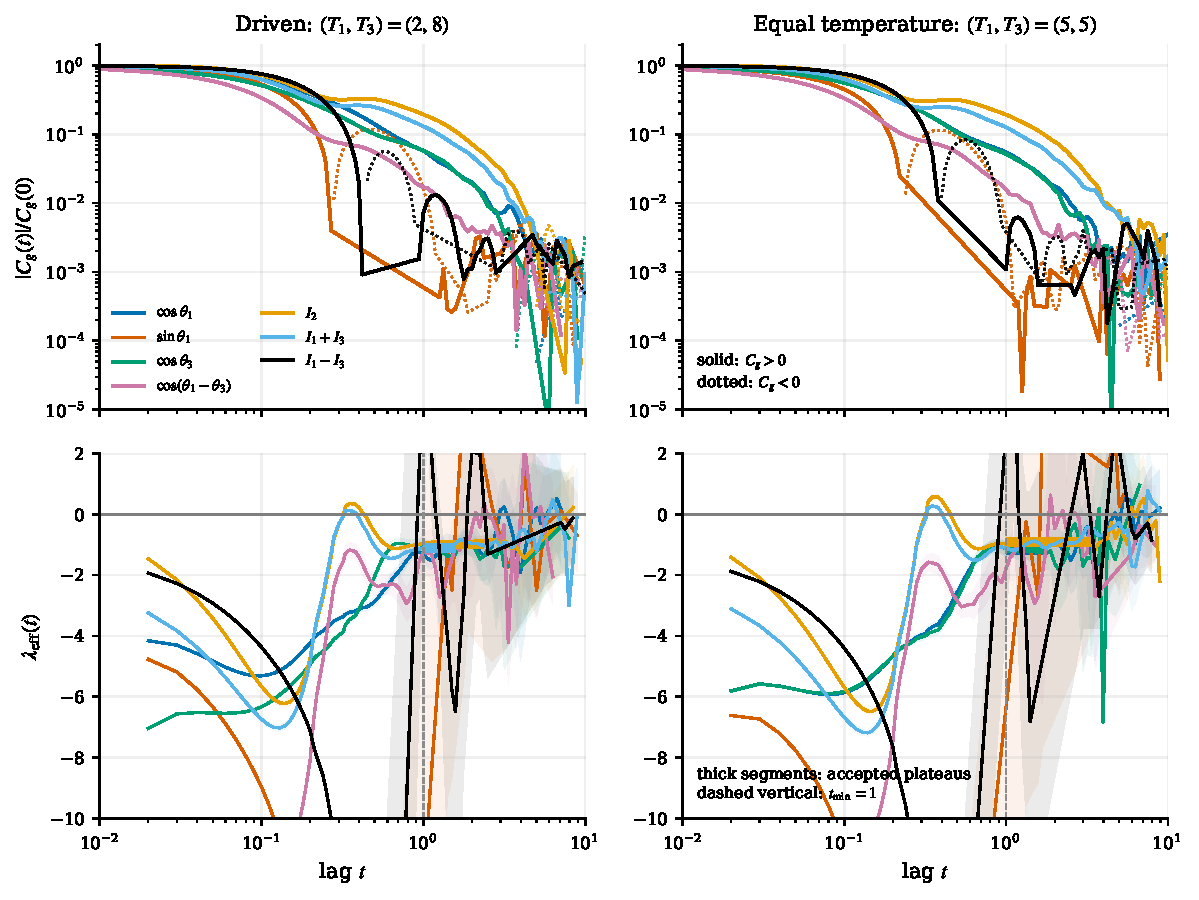
\includegraphics[width=\textwidth]{../figures/stationary_autocorrelation_rates.pdf}
\caption{Top: stationary autocorrelations normalized by $C_g(0)$ on a
logarithmic magnitude axis. Solid portions are positive and dotted portions
negative. Bottom: local decay rates with trajectory-bootstrap 95\% bands.
Thick line segments mark intervals accepted by the frozen plateau rule. The
rapidly growing bands show where the correlation has entered its noise floor.}
\end{figure}

\section*{Driven result}
\begin{table}[h]
\centering\small
\begin{tabular}{lrrrrr}
\toprule
$g$ & $C_g(0)$ & plateau & $\lambda_R$ & 95\% CI & $N_{\rm eff}$\\
\midrule
$\cos\theta_1$ & 0.4794 & \NA & \NA & \NA & \NA\\
$\sin\theta_1$ & 0.4679 & \NA & \NA & \NA & \NA\\
$\cos\theta_3$ & 0.4872 & \NA & \NA & \NA & \NA\\
$\cos(\theta_1-\theta_3)$ & 0.4999 & \NA & \NA & \NA & \NA\\
$I_2$ & 2.6107 & $[1.12,2.37]$ & $-0.9926$ & $[-1.0517,-0.9337]$ & 56,442\\
$I_1+I_3$ & 3.1273 & $[1.00,1.58]$ & $-1.1088$ & $[-1.2013,-1.0228]$ & 74,921\\
$I_1-I_3$ & 5.1962 & \NA & \NA & \NA & \NA\\
\bottomrule
\end{tabular}
\end{table}

Only two observables pass, below the predeclared minimum of three.  Moreover,
the remaining correlations either change sign or lose $3\,\mathrm{SE}$ support
before a stable late interval emerges.  The driven result is therefore
\emph{observable-specific plateaus, no common plateau}.

\section*{Equal-temperature reference}
\begin{table}[h]
\centering\small
\begin{tabular}{lrrrrr}
\toprule
$g$ & $C_g(0)$ & plateau & $\lambda_R$ & 95\% CI & $N_{\rm eff}$\\
\midrule
$\cos\theta_1$ & 0.4879 & $[1.00,1.78]$ & $-1.1878$ & $[-1.3607,-1.0160]$ & 122,898\\
$\sin\theta_1$ & 0.4787 & \NA & \NA & \NA & \NA\\
$\cos\theta_3$ & 0.4863 & $[1.00,1.68]$ & $-1.1334$ & $[-1.3366,-0.9465]$ & 126,444\\
$\cos(\theta_1-\theta_3)$ & 0.4998 & \NA & \NA & \NA & \NA\\
$I_2$ & 2.4254 & $[1.00,3.35]$ & $-0.9065$ & $[-0.9665,-0.8442]$ & 54,591\\
$I_1+I_3$ & 3.0387 & \NA & \NA & \NA & \NA\\
$I_1-I_3$ & 4.9834 & \NA & \NA & \NA & \NA\\
\bottomrule
\end{tabular}
\end{table}

Three observables pass separately, but the estimates span $-1.188$ to
$-0.907$, exceed the allowed 20\% spread, and have no common 95\% CI
intersection.  Hence the equilibrium common-plateau gate also fails.

An important correction to the proposed control is that Gibbs invariance does
not make this full generator self-adjoint: its Hamiltonian Liouville component
is skew-adjoint in Gibbs $L^2$.  Consequently an equilibrium autocorrelation
need not be everywhere positive or monotone.  We report sign changes and
monotonicity violations in the raw diagnostics, but do not misclassify them as
automatic numerical artefacts.

For completeness, the raw equal-temperature diagnostics are:
\begin{table}[h]
\centering\small
\begin{tabular}{lrrr}
\toprule
$g$ & significant rises & supported negative lags & first negative $t$\\
\midrule
$\cos\theta_1$ & 11 & 0 & \NA\\
$\sin\theta_1$ & 85 & 78 & 0.24\\
$\cos\theta_3$ & 5 & 0 & \NA\\
$\cos(\theta_1-\theta_3)$ & 24 & 0 & \NA\\
$I_2$ & 18 & 0 & \NA\\
$I_1+I_3$ & 18 & 0 & \NA\\
$I_1-I_3$ & 81 & 53 & 0.40\\
\bottomrule
\end{tabular}
\caption{Equal-temperature sign and monotonicity diagnostics. A ``significant
rise'' means an adjacent-lag increase larger than the propagated standard
error; a supported negative lag has $C_g<0$ with $|C_g|/\mathrm{SE}\ge3$.
These are descriptive diagnostics, not rejection gates for the non-reversible
Hamiltonian-plus-bath generator.}
\end{table}

\section*{Burn-in and effective support}
All fourteen normalized RMS differences between the full measured trajectory
and the same calculation after deleting its first quarter are below 0.004,
against the frozen 0.05 gate.
\begin{figure}[h]
\centering
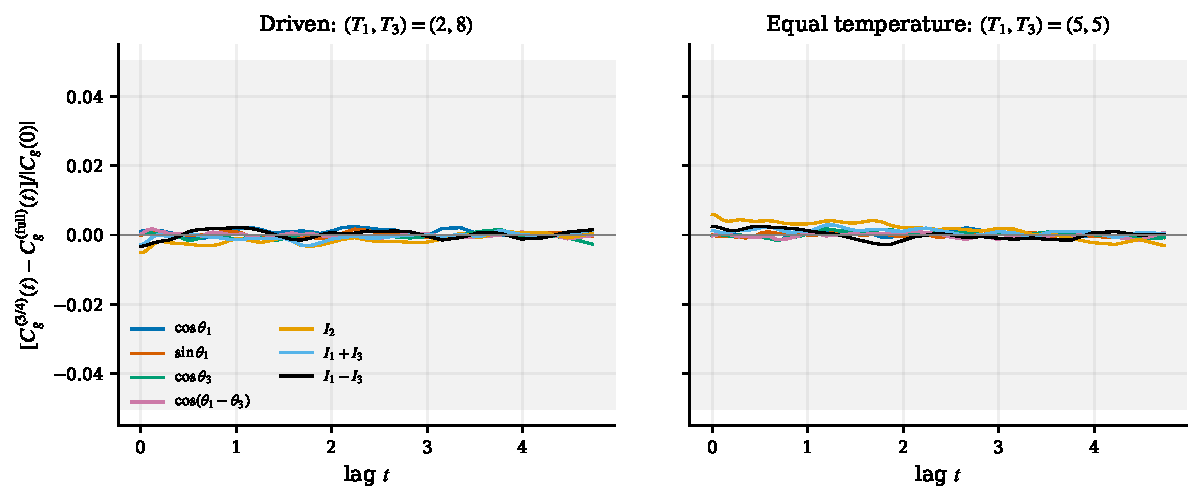
\includegraphics[width=0.95\textwidth]{../figures/stationarity_discard_check.pdf}
\caption{Burn-in check.  Differences between full-measurement correlations and
correlations after deleting the first quarter, normalized by $|C_g(0)|$.  The
grey region is the predeclared $\pm5\%$ stationarity tolerance.}
\end{figure}
The integrated-autocorrelation estimate gives more than 50,000 effective
samples for every accepted plateau.  The failure to find a common rate is thus
not a small-effective-sample failure; it is caused by observable dependence and
loss of late-time signal.

\section*{Damped-oscillation check}
We fitted
\[
C(t)=e^{\lambda_Rt}\{A\cos(\lambda_It)+B\sin(\lambda_It)\}
\]
on the predeclared late support.  No observable has a resolved nonzero
$\lambda_I$: every candidate either fails the half-cycle resolution condition,
fails to improve AIC by 10 over the nested real exponential, or lacks enough
supported points.  In particular, the driven $\sin\theta_1$ unconstrained
optimum is $\lambda_I=7.02$ with bootstrap interval approximately
$[0,10.81]$, but the damped model has $\Delta\mathrm{AIC}=+1.43$ and is not
accepted.

\begin{table}[h]
\centering\scriptsize
\begin{tabular}{llrrrl}
\toprule
case & $g$ & fitted $\lambda_I$ & 95\% CI & half-cycle threshold & verdict\\
\midrule
driven & $\cos\theta_1$ & $1.3\!\times\!10^{-10}$ & $[2.8\!\times\!10^{-11},2.1\!\times\!10^{-5}]$ & 1.138 & not resolved\\
driven & $\sin\theta_1$ & 7.019 & $[3.0\!\times\!10^{-6},10.815]$ & 1.054 & AIC fails\\
driven & $\cos\theta_3$ & $4.0\!\times\!10^{-10}$ & $[4.3\!\times\!10^{-11},0.0133]$ & 1.579 & not resolved\\
driven & $\cos(\theta_1-\theta_3)$ & $8.0\!\times\!10^{-7}$ & $[1.8\!\times\!10^{-10},0.0037]$ & 1.893 & not resolved\\
driven & $I_2$ & $7.8\!\times\!10^{-8}$ & $[3.9\!\times\!10^{-10},0.0055]$ & 1.054 & not resolved\\
driven & $I_1+I_3$ & $7.3\!\times\!10^{-9}$ & $[3.9\!\times\!10^{-11},0.0049]$ & 1.054 & not resolved\\
driven & $I_1-I_3$ & \NA & \NA & \NA & insufficient support\\
\midrule
equilibrium & $\cos\theta_1$ & $1.6\!\times\!10^{-10}$ & $[1.3\!\times\!10^{-12},0.0064]$ & 1.454 & not resolved\\
equilibrium & $\sin\theta_1$ & \NA & \NA & \NA & insufficient support\\
equilibrium & $\cos\theta_3$ & 0.0015 & $[8.9\!\times\!10^{-11},0.0073]$ & 1.579 & not resolved\\
equilibrium & $\cos(\theta_1-\theta_3)$ & $7.6\!\times\!10^{-9}$ & $[2.0\!\times\!10^{-10},0.0015]$ & 1.454 & not resolved\\
equilibrium & $I_2$ & 0.00019 & $[5.6\!\times\!10^{-11},0.00040]$ & 0.905 & not resolved\\
equilibrium & $I_1+I_3$ & $3.4\!\times\!10^{-7}$ & $[1.1\!\times\!10^{-9},3.4\!\times\!10^{-5}]$ & 0.680 & not resolved\\
equilibrium & $I_1-I_3$ & \NA & \NA & \NA & insufficient support\\
\bottomrule
\end{tabular}
\caption{Damped-fit frequencies.  A frequency is accepted only if the interval
contains at least half a cycle and the damped model improves AIC by at least
10 over the nested real exponential. None passes.}
\end{table}

The machine-readable values, including $\lambda_R$, bootstrap acceptance and
$\Delta\mathrm{AIC}$, are in \path{analysis/*_damped_fits.csv}.  This
supports an essentially real resolved late decay, but not a unique real gap.

\section*{Comparison with the previous numbers}
The two driven plateaus, $-0.993$ and $-1.109$, are closest to the historical
full-window diagnostic $-0.934$.  They do not reproduce the early-window and
Prony values $-1.60$ and $-1.65$, and the data do not support interpreting
$-0.68$ as a common late-time plateau.  The correct replacement sentence is:
\begin{quote}
Stationary autocorrelations resolve observable-specific rates of order $-1$,
but no common late-time plateau across observables; the spectral gap remains
numerically unresolved.
\end{quote}

\section*{Numerical caveat and provenance}
No trajectory became non-finite.  The inherited floor was nevertheless
activated 91,674 times in the driven case and 97,047 times at equilibrium, so
this experiment estimates the spectrum of the stated discretized dynamics and
does not remove that historical numerical caveat.

The frozen source commit is
\path{b238c2fff9e5f9366cb2c8bafddcef90f7da5b12}; its remote cherry-pick is
\path{db022529c1d8e4e4d1153742018a088d8be3264b}.  Sampler source SHA-256 is
\path{a1d558c267a4eca00c3b8f445e1236c1d097be50e72845f18ed4a4e12d7c9df1};
binary SHA-256 is
\path{447ba1141ba5f126bccd6f39661c939eee4683ef96fcd12a1595420e7e532316}.
Base seeds are 2026090701 and 2026090702, with stream seed equal to base plus
stream ID.  Exact commands and complete hashes are under \path{provenance/};
the raw correlation tables are \path{analysis/*_autocorrelations.csv}.

\end{document}
